
\PassOptionsToPackage{dvipsnames,table,usenames,svgnames}{xcolor}
\documentclass[a4paper, 10pt, openright,twoside,onecolumn]{memoir}

\usepackage{asymptote}
\def\asydir{asydir}

\usepackage{marginnote}
\def\blank#1{\rule{#1}{0.5pt}}


\usepackage{lipsum}
\usepackage{tikz}
\usepackage{xcolor}
\usepackage{pgfplots}
\pgfplotsset{compat=1.18}
\usetikzlibrary{calc}

% ==> language
\usepackage[no-math]{fontspec}
\usepackage{fontawesome}
\usepackage[Khmer, Latin]{ucharclasses}
\usepackage{etoolbox}
\usepackage{enumitem}

% ==> main font
\setmainfont[
	BoldFont = Khmer OS Bokor,
	ItalicFont = Khmer OS Metal Chrieng,
	BoldItalicFont = Khmer OS Muol,
	SmallCapsFont = TeX Gyre Pagella,
	Script=Khmer,Scale=1
]{Khmer OS Siemreap}

\XeTeXlinebreaklocale "kh"
\XeTeXlinebreakskip = 0pt plus 1pt minus 1pt


\newfontfamily{\khmerfamily}
[
	BoldFont = Khmer OS Bokor,
	ItalicFont = Khmer OS Metal Chrieng,
	BoldItalicFont = Khmer OS Muol,
	SmallCapsFont = TeX Gyre Pagella,
	Script=Khmer,Scale=1
]{Khmer OS Siemreap}
\newfontfamily{\englishfamily}{TeX Gyre Pagella}[Ligatures=TeX, Scale=1.1] %Simonetta
\newfontfamily{\monofamily}[Scale=1]{Latin Modern Mono}
\newfontfamily{\latinfamily}[Scale=1.3]{Latin Modern Roman}

% Define new font family (have to)   <-- BUG
\newrobustcmd{\englishfont}{\englishfamily\let\currentenglish\englishfamily }
\newrobustcmd{\khmerfont}{\khmerfamily\let\currentkhmer\khmerfamily}
\newrobustcmd{\mono}{\monofamily\let\currentenglish\monofamily }
\newrobustcmd{\en}{\latinfamily\let\currentenglish\latinfamily}

% Initialize fonts
\khmerfont\englishfont
\setTransitionsForLatin{\currentenglish}{\currentkhmer}

% Change typewriter font family
\renewcommand{\ttfamily}{\mono}
% <==
% ==> Fixed: math font

% change bold face
\usepackage{bbold}
\let\altmathbb\mathbb
\AtBeginDocument{\let\mathbb\altmathbb}

% use mathpazo, instead of default font
\let\temp\rmdefault
\usepackage{mathpazo}
\let\rmdefault\temp
% <==
% ==> khmer fonts
\newcommand{\kml}{
	\fontspec[ Script=Khmer, Scale=1,AutoFakeBold=1, AutoFakeSlant=0.25] 
	{Khmer OS Muol}\selectfont
}
\newcommand{\kpali}{
	\fontspec[ Scale=1, Script=Khmer,AutoFakeBold=1, AutoFakeSlant=0.25] 
	{Khmer OS Muol Pali}\selectfont
}
\newcommand{\kbk}{
	\fontspec[Script=Khmer, Scale=1.125,AutoFakeBold=1, AutoFakeSlant=0.25]
	{Khmer OS Bokor}\selectfont
}
\newcommand{\kmetal}{
	\fontspec[Script=Khmer, Scale=1.125,AutoFakeBold=1, AutoFakeSlant=0.25]
	{Khmer OS Metal Chrieng}\selectfont
}


% useful khmer-math shortcuts
\def\KHstop{\quad\text{។}}
\def\KHor{\quad\text{ឬ}\quad}
\def\KHand{\quad\text{និង}\quad}
% <==
% ==> khmer counter
%khmer number

\makeatletter
\def\khmer#1{\expandafter\@khmer\csname c@#1\endcsname}
\def\@khmer#1{\expandafter\@@khmer\number#1\@nil}
\def\@@khmer#1{%
	\ifx#1\@nil% terminate when encounter @nil
	\else%
	\ifcase#1 ០\or ១\or ២\or ៣\or ៤\or ៥\or ៦\or ៧\or ៨\or ៩\fi%
	\expandafter\@@khmer% recursively map the following characters
	\fi}

% khmer alphabet
\def\khmernumeral#1{\@@khmer#1\@nil}
\def\alpkh#1{\expandafter\@alpkh\csname c@#1\endcsname}
\def\@alpkh#1{%
	\ifcase#1% zero -> none
	\or ក\or ខ\or គ\or ឃ\or ង%
	\or ច\or ឆ\or ជ\or ឈ\or ញ%
	\or ដ\or ឋ\or ឌ\or ឍ\or ណ%
	\or ត\or ថ\or ទ\or ធ\or ន%
	\or ប\or ផ\or ព\or ភ\or ម%
	\or យ\or រ\or ល\or វ\or ស%
	\or ហ\or ឡ\or អ%
	\else%[most]
	\@ctrerr % otherwise, counter error!
	\fi}
\makeatother

%declare new enumerate counter
\AddEnumerateCounter{\alpkh}{\@alpkh}{ឈ}
\AddEnumerateCounter{\khmer}{\@khmer}{៣}
% <==

% <==
% ==> redefine the names
\def\chaptername{ជំពូកទី}
\def\axiomName{ស្វ័យសត្យ}
\def\definitionName{និយមន័យ}
\def\theoremName{ទ្រឹស្តីបទ}
\def\lemmaName{បទគន្លឹះ}
\def\propositionName{សំណើ}
\def\corollaryName{វិបាក}
\def\exampleName{ឧទាហរណ៍}
\def\exerciseName{លំហាត់}
\def\proofName{សម្រាយបញ្ជាក់}
\def\solutionName{ដំណោះស្រាយ}
\def\remarkName{សម្គាល់}
% <==
% ==> math
\usepackage{amsmath, amsthm, amsfonts, amssymb}
\usepackage{mathtools}

\mathtoolsset{centercolon} % not work when using |mathpazo|
\DeclarePairedDelimiter\abs{\lvert}{\rvert}
\DeclarePairedDelimiterX\norm[1]\lVert\rVert{
	\ifblank{#1}{\:\cdot\:}{#1}
}
\def\set#1#2{\left\{#1 ~:~ #2\right\}}
\def\permil{\text{\hskip 0.3pt\englishfont\textperthousand}}


\DeclareMathOperator{\arccot}{cot}
\DeclareMathOperator{\arcsec}{arcsec}
\DeclareMathOperator{\arccsc}{arccsc}

\DeclareMathOperator{\asinh}{argsh}
\DeclareMathOperator{\acosh}{argch}
\DeclareMathOperator{\atanh}{argtanh}
\DeclareMathOperator{\acoth}{argcoth}

\DeclareMathOperator{\lcm}{lcm}
\DeclareMathOperator{\ord}{ord}
\DeclareMathOperator{\sym}{sym}
\DeclareMathOperator{\tr}{trace}
\DeclareMathOperator{\dom}{dom}
\DeclareMathOperator{\ran}{ran}
\DeclareMathOperator{\id}{id}
\DeclareMathOperator{\card}{card}




\def\N{\mathbb{N}}
\def\Z{\mathbb{Z}}
\def\Q{\mathbb{Q}}
\def\Qc{\mathbb{Q}^{\complement}}
\def\R{\mathbb{R}}
\def\C{\mathbb{C}}
\def\F{\mathbb{F}}
\def\K{\mathbb{K}}
\def\P{\mathbb{P}}
\def\Nx{\mathbb{N}[x]}
\def\Zx{\mathbb{Z}[x]}
\def\Qx{\mathbb{Q}[x]}
\def\Rx{\mathbb{R}[x]}
\def\Cx{\mathbb{C}[x]}

\def\S{\mathcal{S}}
\def\labelitemi{$\circ$}
\def\inv{^{-1}}
\def\ang#1{\left\langle#1\right\rangle}
\def\inner#1{\left\langle#1\right\rangle}
\def\tran{^\mathrm{T}}
%\renewcommand{\d}{\frac{d}{dx}}
\renewcommand{\vec}[1]{\mathbf{#1}}
% <==
% ==> listings
\usepackage{xcolor}
\usepackage{listings}
% ==> basic
\lstset{%
	basicstyle=\small\ttfamily,
	keywordstyle=\color{black},
	commentstyle=\color{gray},
	keywordstyle=[1]{\color{blue!90!black}},
	keywordstyle=[2]{\color{magenta!90!black}},
	keywordstyle=[3]{\color{red!60!orange}},
	keywordstyle=[4]{\color{teal}},
  keywordstyle=[5]{\color{magenta!90!black}}, % <-- otherkeywords, BUG
	commentstyle=\color{gray},
	stringstyle=\color{green!60!black},
	tabsize=2,
	%
	numbers=none,
	numberstyle=\tiny\color{blue!70!gray},
	stepnumber=1,
	%
	frame=Lt,
	breaklines=true,
	xleftmargin=0cm,
	rulecolor=\color{gray!50!black},
	aboveskip=0.5cm,
	belowskip=0.5cm
}
% <==
% ==> code c
\lstdefinelanguage{cmeng}{
  morekeywords={
    auto,break,case,char,const,continue,default,do,double,%
    else,enum,extern,float,for,goto,if,int,long,register,return,%
    short,signed,sizeof,static,struct,switch,typedef,union,unsigned,%
    void,volatile,while},%
  morekeywords=[2]{
    printf, scanf,  include
  },
  otherkeywords={\#,<,>,\&},
  morekeywords=[5]{\#,<,>,\&},
  sensitive,%
	morecomment=[l]{//},
	morecomment=[s]{/*}{*/},
	morestring=[b]',
	morestring=[b]",
}
% <==
% ==> code python
\lstdefinelanguage{py}{
	morekeywords={
		access,and,as,break,class,continue,def,del,elif,else,
		except,exec,finally,for,from,global,if,import,in,is,lambda,
		not,or,pass,print,raise,return,try,while},
	% Built-ins
	morekeywords=[2]{
		abs,all,any,basestring,bin,bool,bytearray,
		callable,chr,classmethod,cmp,compile,complex,delattr,dict,dir,
		divmod,enumerate,eval,execfile,file,filter,float,format,
		frozenset,getattr,globals,hasattr,hash,help,hex,id,input,int,
		isinstance,issubclass,iter,len,list,locals,long,map,max,
		memoryview,min,next,object,oct,open,ord,pow,property,range,
		raw_input,reduce,reload,repr,reversed,round,set,setattr,slice,
		sorted,staticmethod,str,sum,super,tuple,type,unichr,unicode,
		vars,xrange,zip,apply,buffer,coerce,intern,True,False},
	%
	morecomment=[l]\#,%
	morestring=[b]',%
	morestring=[b]",%
	morecomment=[s]{'''}{'''},% used for documentation text
	%                         % (mulitiline strings)
	morecomment=[s]{"""}{"""},% added by Philipp Matthias Hahn
	morestring=[s]{r'}{'},% `raw' strings
	morestring=[s]{r"}{"},%
	morestring=[s]{r'''}{'''},%
	morestring=[s]{r"""}{"""},%
	morestring=[s]{u'}{'},% unicode strings
	morestring=[s]{u"}{"},%
	morestring=[s]{u'''}{'''},%
	morestring=[s]{u"""}{"""},%
	%
	sensitive=true,%
}
% <==
% ==> code asy
\lstdefinelanguage{asy}{ %% Added by Sivmeng HUN
	morekeywords=[1]{
		import, for, if, else,new, do,and, access,
		from, while, break, continue, unravel, 
		operator, include, return},
	morekeywords=[2]{
		struct,typedef,static,public,readable,private,explicit,
		void,bool,int,real,string,var,picture,
		pair, path, pair3, path3, triple, transform, guide, pen, frame
	},
	morekeywords=[3]{
		true,false,and,cycle,controls,tension,atleast,
		curl,null,nullframe,nullpath,
		currentpicture,currentpen,currentprojection,
		inch,inches,cm,mm,pt,bp,up,down,right,left,
		E,N,S,W,NE,NW,SE,SW,
		solid,dashed,dashdotted,longdashed,longdashdotted,
		squarecap,roundcap,extendcap,miterjoin,roundjoin,
		beveljoin,zerowinding,evenodd,invisible
	},
	morekeywords=[4]{
		size,unitsize,draw,dot,label,
		sqrt,sin,cos,tan,cot,Sin,Cos,Tan,Cot,
		graph,
	},
	%
	morecomment=[l]{//},
	morecomment=[s]{/*}{*/},
	morestring=[b]',
	morestring=[b]",
	%
}
% <==
% <==
% ==> mdframe theorem
\usepackage{thmtools}
\usepackage[framemethod=TikZ]{mdframed}

% ==> Axiom
\mdfdefinestyle{mdAxiomStyle}{
	roundcorner = 10pt,
	linewidth=1.125pt,
	skipabove=12pt,
	innerbottommargin=9pt,
	skipbelow=2pt,
	nobreak=true,
	linecolor=blue,
	backgroundcolor=TealBlue!5,
}
\declaretheoremstyle[
	headfont=\bfseries\color{MidnightBlue},
	bodyfont=\itshape,
	mdframed={style=mdAxiomStyle},
	headpunct={\\[3pt]},
	postheadspace={0pt},
	notefont=\bfseries\itshape\color{gray!50!blue},
	notebraces={~(}{)},
]{mdAxiom}
% <==
% ==> Definition
\mdfdefinestyle{mdDefinitionStyle}{
	roundcorner = 10pt,
	linewidth=1.125pt,
	skipabove=12pt,
	innerbottommargin=9pt,
	skipbelow=2pt,
	nobreak=true,
	linecolor=blue,
	backgroundcolor=TealBlue!5,
}
\declaretheoremstyle[
	headfont=\bfseries\color{MidnightBlue},
	bodyfont=\itshape,
	mdframed={style=mdDefinitionStyle},
	headpunct={\\[3pt]},
	postheadspace={0pt},
	notefont=\bfseries\itshape\color{gray!50!blue},
	notebraces={~(}{)},
]{mdDefinition}
% <==
% ==> Theorem
\mdfdefinestyle{mdTheoremStyle}{%
	linewidth=1pt,
	skipabove=12pt,
	frametitleaboveskip=5pt,
	frametitlebelowskip=0pt,
	skipbelow=2pt,
	innertopmargin=5pt,
	innerbottommargin=8pt,
	nobreak=true,
	linecolor=RawSienna!40,
	backgroundcolor=Salmon!10,
}
\declaretheoremstyle[
	headfont=\bfseries\color{RawSienna},
  headindent=0pt,
	bodyfont=\itshape,
	mdframed={style=mdTheoremStyle},
	notefont=\normalfont\itshape\small\color{RawSienna},
	notebraces={~$\big\langle$}{$\big\rangle$},
	headpunct={\\[3pt]},
	postheadspace={0pt},
]{mdTheorem}
% <==
% ==> Exercise
\mdfdefinestyle{mdExerciseStyle}{%
	skipabove=5pt,
	skipbelow=5pt,
	linewidth=1pt,
	rightline=true,
	leftline=true,
	topline=true,
	bottomline=true,
	linecolor=blue,
	backgroundcolor=white
}
\declaretheoremstyle[
	headfont=\bfseries\color{blue},
	bodyfont=\normalfont,
	headindent=0pt,
	spaceabove=2pt,
	spacebelow=5pt,
	mdframed={style=mdExerciseStyle},
	notefont=\small\bfseries\itshape\color{DarkGreen},
	notebraces={~(}{)},
	headpunct={ },
]{mdExercise}

% <==
% ==> Proof
\declaretheoremstyle[
	spaceabove=6pt,
	spacebelow=6pt,
	headindent=0pt,
	headfont=\normalfont\color{magenta!70!blue},
	bodyfont = \normalfont,
	postheadspace=1em,
	qed=$\color{magenta!70!black}\blacksquare$,
	headpunct={ },
]{mdProof}
% <==

% ==> Declaring the theorems
\declaretheorem{axiom}[style=mdAxiom, name={\kml\axiomName}, numberwithin=chapter]
\declaretheorem[style=mdDefinition, name={\kml\definitionName}, sibling=axiom]{definition}

\declaretheorem{theorem}[style=mdTheorem, name={\theoremName},numberwithin=chapter]
\declaretheorem{lemma}[style=mdTheorem, name={\lemmaName},sibling=theorem]
\declaretheorem{proposition}[style=mdTheorem, name={\propositionName}, sibling=theorem]
\declaretheorem{corollary}[style=mdTheorem, sibling=theorem, name={\corollaryName}]

\declaretheorem{example}[name={\exampleName},style=mdExercise, numberwithin=section]
\declaretheorem{exercise}[name={\exerciseName},style=mdExercise, sibling=example]

%\newenvironment{problem}{\begin{exercise}}{\end{exercise}}

%% Proof
\declaretheorem[name={\bfseries\proofName},numbered=no,style=mdProof]{Proof}
\renewenvironment{proof}{\begin{Proof}}{\end{Proof}}
\declaretheorem[name={\itshape\solutionName},numbered=no,style=mdProof]{solution}
% <==
% <==
% ==> tweaking memmoir
\checkandfixthelayout
%\setlrmarginsandblock{2cm}{8cm}{*}
%\setulmarginsandblock{3cm}{*}{1.5}


\makepagestyle{myruled}
\makeheadrule {myruled}{\textwidth}{\normalrulethickness}
\makefootrule {myruled}{\textwidth}{\normalrulethickness}{\footruleskip}
\makeevenhead {myruled}{}{\small\itshape\leftmark} {}
\makeoddhead  {myruled}{}{\small\itshape\rightmark}{}
\makeevenfoot {myruled}{}{\small\thepage} {}
\makeoddfoot  {myruled}{}{\small\thepage} {}

\makeatletter % because of \@chapapp
\makepsmarks{myruled}{
  \nouppercaseheads
  \createmark{chapter}{both}{shownumber}{}{. \space}
  \createmark{section}{right}{shownumber}{}{. \space}
  \createmark{subsection}{right}{shownumber}{}{. \space}
  \createmark{subsubsection}{right}{shownumber}{}{. \ }
  \createplainmark {toc} {both} {\contentsname} 
  \createplainmark {lof} {both} {\listfigurename}
  \createplainmark {lot} {both} {\listtablename} 
  \createplainmark {bib} {both} {\bibname} 
  \createplainmark {index} {both} {\indexname} 
  \createplainmark {glossary} {both} {\glossaryname}
}
\makeatother
\setsecnumdepth{subsubsection}
\pagestyle{myruled}

\renewcommand{\headheight}{17pt}
% <==


% \setlength{\arrayrulewidth}{0.5pt} 
\setlength{\tabcolsep}{5pt}
\renewcommand{\arraystretch}{1.65}

\begin{document}
	
\chapter{Operation Research}

\section{Linear Programming}

\begin{exercise}
	អ្នកគណនីយម្នាក់ត្រៀមប្រមូលពន្ធសម្រាប់ការងារបុគ្គល និងការងារជាក្រុម ។
  ជាមធ្យម ចំពោះការងារបុគ្គលនាងត្រូវការពេល 3h ហើយត្រូវការប្រើកុំព្យូទ័រ 1h ។
  ​ចំណែកឯការងារជាក្រុមវិញនាងត្រូវការពេល 4h ហើយត្រូវការប្រើកុំព្យូទ័រ 2h ។
  ដោយសារតែនាងជាប់រវល់ នាងមានពេលតែ 240h តែប៉ុណ្ណោះ
  ហើយនាងអាចប្រើកុំព្យូទ័របានតែ 100h ប៉ុណ្ណោះ ។ បើសិនជានាងអាចរកប្រាក់បាន
  \$80 ចំពោះការងារបុគ្គល ហើយអាចរកបាន \$150 ចំពោះការងារជាក្រុម
  តើនាងត្រូវប្រើវិធីសាស្ត្រយ៉ាងណាដើម្បីឱ្យនាងអាចរកប្រាក់បានច្រើនបំផុត ។
\end{exercise}
\begin{solution}
  \text{}
	\begin{center}
    \begin{tabular}{l c c c}
      \toprule
      {}         &ការងារបុគ្គល    &ការងារជាក្រុម   &ពេលត្រូវាការ \\
      \cmidrule(r){2-2}
      \cmidrule(r){3-3}
      \cmidrule(r){4-4}
      ពេលរបស់នាង &3            &4           &240h\\
      ពេលកុំព្យូទ័រ   &1            &2           &100h\\
      \hline
      ប្រាក់ចំណូល  &\$80         &\$80         &{}\\
      \bottomrule
    \end{tabular}
  \end{center}
  យើងតាង $x$ ជាចំនួនការងារបុគ្គល  ហើយ $y$ ជាចំនួនការងារជាក្រុមដែលនាងទទួលធ្វើ ។
  យើងបានសមីការគោលដៅ (objective function) គឺ $P(x,y) = 80x+150y$ ។
  យើងបានប្រព័ន្ធសមីការដូចតទៅ
  \begin{align*}
  	\begin{cases}
    	x\geq 0\\
      y\geq 0\\
      3x+4y \leq 240\\
      x+2y \leq 100
    \end{cases}
  \end{align*}
  ដោះស្រាយប្រព័ន្ធវិសមីការខាងលើយ
  \begin{center}
  	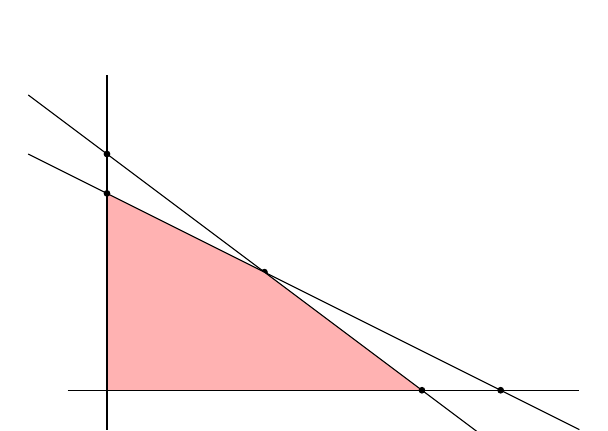
\begin{tikzpicture}
      %
      \draw[fill=black] (2, 1.5) circle (1pt);
      \fill[red!30] (0,0)--(4,0)--(2,1.5)--(0,2.5)--cycle;

    	\draw (-0.5,0) -- (6,0);
      \draw (0,-0.5) -- (0,4);

      % 3x+4y=240
      % y = (-3/4)x + 3
      \draw[fill=black] (0,3) circle (1pt);
      \draw[fill=black] (4,0) circle (1pt);
      \draw (-1, 15/4)--(5, -3/4);

      % x+2y = 100
      % y = (-1/2)x +5/2
      \draw[fill=black] (0,2.5) circle (1pt);
      \draw[fill=black] (5,0) circle (1pt);
      \draw (-1, 3) -- (6,-1/2);
    \end{tikzpicture}
  \end{center}

  យើងឃើញថា
  \begin{center}
    \begin{tabular}{l c}
      \toprule
      ចំណុច       & $P(x,y)=80x+150y$\\
      \cmidrule(r){1-1} \cmidrule(l){2-2}
      $(0,0)$     & $P=0$\\
      $(80,0)$    & $P=6,400$\\
      $(40,30)$   & $P=7,700$\\
      $(0,50)$    & $P=7,500$\\
      \bottomrule
    \end{tabular}
  \end{center}
  ដូចនេះ តម្លៃអតិបរមារត្រូវនឹងចំណុច $(40,30)$ ។
\end{solution}



\newpage
\section{Assignment}
ក្រុមហ៊ុនផលិតរថយន្ត Automobile Alliance មានគម្រោងរៀបចំផលិតរថយន្តជា ៣
ប្រភេទ ៖ ប្រភេទរថយន្តដឹកទំនិញ (truck), ប្រភេទរថយន្តខ្នាតតូច (small cars),
និងប្រភេទរថយន្តបែបប្រណិត (luxury cars) ។ រោងចក្រតម្លើងរថយន្តនៅក្រៅ Detroit
រដ្ឋ Michigan ទទួលតម្លើងរថយន្តបែបប្រណិតចំនួន ២ ម៉ូដ ។

\paragraph{Auto Assembly and Luxury cars:}
ម៉ូតទី ១ គឺប្រភេទ Family Thrillseeker ដែលមានទ្វារបួន អមជាមួយនឹងកៅអីស្រោបដោយ vinyl
ផ្នែកខាងក្នុងគ្របដោយផ្លាស្ទិក ប្រភេទស្តង់ដារ និងមានប្រព័ន្ធហ្គាសដ៏ល្អ ។
រថយន្តប្រភេទនេះត្រូវបានគេប្រូម៉ូតថាជាជម្រើសល្អសម្រាប់គ្រួសារដែលមានធនធានល្អល្មម
ហើយក្រុមហ៊ុនអាចរកចំណូលដោយការលក់រថយន្តប្រភេទនេះក្រោមតម្លៃ \$3,600 ក្នុងមួយគ្រឿង ។

ប្រភេទម៉ូតទី ២ មានឈ្មោះថា Classy Cruiser ដែលជារថយន្តប្រភេទ sedan ទ្វារពីរ
អមជាមួយនឹងកៅអីអង្គុយស្រោមដោយស្បែកសត្វ ផ្នែកខាងក្នុងគ្របដណ្តប់ដោយឈើប្រណិត
ហើយមានបច្ចេកវិទ្យា GPS ព្រមទាំងមានលក្ខណៈពិសេសៗជាច្រើនទៀត ។
វាត្រូវបានគេប្រូម៉ូតថាជាជម្រើសល្អបំផុតសម្រាប់គ្រួសារថ្នាក់កណ្តាល និងថ្នាក់ខ្ពស់
ហើយរថយន្តប្រភេទនេះអាចរកប្រាក់ចំណូលឱ្យក្រុមហ៊ុនប្រមាណ \$5,400 ក្នុងមួយគ្រឿង ។

ប្រធានអ្នកគ្រប់គ្រងផ្នែកតម្លើង អ្នកស្រី Rachel Rosencrantz គឺកំពុងតែសម្រេចចិត្តក្នុងការតម្លើងរថយន្តទាំងពីរម៉ូតនេះ
សម្រាប់ខែក្រោយ ។ អ្នកស្រីត្រូវសម្រេចចិត្តថាតើអ្នកស្រីគួរតម្លើងរថយន្តម៉ូតទាំងពីរនេះចំនួនប៉ុន្មាន
ដើម្បីឱ្យក្រុមហ៊ុនទទួលបានប្រាក់ចំនួនខ្ពស់ ។ អ្នកស្រីដឹងថាក្នុងរោងចក្រតម្លើងរថយន្តនេះមានចំនួនម៉ោងធ្វើការសរុប
48,000h ក្នុងមួយខែ ។ ជាងនេះទៅទៀតគេដឹងថា ចំពោះរថយន្តម៉ូត Family Thrillseeker
មួយគ្រឿងត្រូវការពេលតម្លើងចំនួន 6h ។ ចំណែកឯម៉ូត Cruiser វិញត្រូវការពេល 10.5h ដើម្បីតម្លើង ។
ម៉្យាងទៀតរោថចក្រនេះគ្រាន់តែជារោងចក្រតម្លើង មានន័យថាបំណែកផ្សេងៗទៀតរបស់រថយន្តដូចជា
កញ្ចក់ សំបករថយន្ត ទ្វារ បង្អួច កៅអី និងចង្កូតជាដើម
ត្រូវធ្វើការនាំចូលពីរោងចក្រផ្សេងក្នុងរដ្ឋ Michigan ដើម្បីយកមកតម្លើង ។ 
នៅក្នុងខែក្រោយនេះ មានភាពមិនប្រក្រតីក្នុងក្រុមហ៊ុនផលិតបំណែករថយន្ត ធ្វើឱ្យគេអាចផលិតទ្វារបានតែ
20,000 ប៉ុណ្ណោះ ។ គេដឹងថារថយន្តទាំងម៉ូត Family Thillseeker និងទាំងម៉ូត Classy Cruiser
ប្រើទ្វារប្រភេទដូចគ្នា ។

លើសពីនេះទៅទៀត វាត្រូវបានអ្នកជំនាញឱ្យយោបល់ថារថយន្តម៉ូត Classy Cruiser គួរតែផលិតយ៉ាងច្រើនត្រឹម
3,500 គ្រឿងបានហើយ តែចំពោះថយន្តម៉ូត Thrillseeker មិនបានគេកំណត់ចំនួនទេ ។

\begin{enumerate}[label={\textbf{(\alph*)}}]
\item បង្កើត និងដោះស្រាយចំណោត LP មួយនេះដើម្បីកំណត់ចំនួនរថយន្តប្រភេទ
  Thrill-seeker និងប្រភេទ Cruiser ដែលត្រូវតម្លើង ៖ \\[2cm]
  យើងតាង $x$ ជាចំនួនរថយន្តប្រភេទ Thrillseeker,
  និងតាង $y$ ជាចំនួនរថយន្តប្រភេទ Cruiser ។
  \begin{center}
    \begin{tabular}{lcc}
      \toprule
                &Family Thrillseeker & Classy Cruiser\\
      \cmidrule(r){2-2}\cmidrule(l){3-3}
      ចំនួន & $x>0$ & $0<y<3,500$\\
      ចំណូល       &\$3,600             & \$5,400\\
      ទ្វារ  & 4 & 2\\
      ពេលត្រូវការ &6h                  & 10.5h\\\hline
      ពេលសរុប & \multicolumn{2}{c}{ 48,000h} \\
      ទ្វារសរុប & \multicolumn{2}{c}{20,000 ទ្វារ} \\
      \bottomrule
    \end{tabular}
  \end{center}
  គេចង់ផលិតឡានយ៉ាងណាឱ្យទទួលបានប្រាក់ចំណូលខ្ពស់បំផុត មានន័យថាគេចង់ maximize អនុគមន៍គោលដៅ
  \[P(x,y) = 3,600x + 5,400y\KHstop\]
  ហេតុនេះយើងបាន contraints ដូចខាងក្រោម
  \[
    \begin{cases}
    	4x+2y\leq 20,000\\
      6x+10.5y \leq 48,000\\
      x>0\\
      y>0\\
      y\leq 3,500
    \end{cases}
  \]
  យើងនឹងដោះស្រាយចំណោត LP នេះក្នុងភាសា R:

  \begin{lstlisting}
library(lpSolve)

a_P = c(3600, 5400)
a_constraint = matrix( c(4,2, 6,10.5, 1,0, 0,1, 0,1), ncol=2, byrow=TRUE )
a_dir = c("<=", "<=", ">", ">", "<=")
a_rhs = c(20000, 48000, 0, 0, 3500)

a_result = lp("max", a_P, a_constraint, a_dir, a_rhs)
  \end{lstlisting}
  បន្ទាប់ពីដំណើរការកូដខាងលើយើងបានលទ្ធផល 
  \begin{verbatim}
> a_result
Success: the objective function is 26640000 
> a_result$solution
[1] 3800 2400
  \end{verbatim}
  ដូចនេះមានន័យថា
  \begin{align*}
  	&x_a=3,800\\
    &y_a=2,400\\
    &P_a=26,640,000 
  \end{align*}

 
 \item នាយកដ្ឋានផ្នែកទីផ្សារបានឱ្យដឹងថាក្រុមហ៊ុនអាចចំណាយប្រាក់ $\$500,000$
   ក្នុងយុធ្ធនាការសម្រាប់ធ្វើការផ្សព្វផ្សាយ ដែលនឹងធ្វើឱ្យតម្រូវការរថយន្ត Classy Cruiser កើនឡើងបាន
   $20\%$ ក្នុងខែក្រោយ ។ តើគួរតែធ្វើយុទ្ធនាការបែបនេះឬទេ ?\\[2cm]

   បើយុនធ្ធនាការបែបនេះកើតឡើងមែន នោះតម្រូវការរថយន្ត Classy Cruiser នឹងកើនដល់ (ខ្ពស់បំផុត)
   គឺ $3500\times 1.20=4,200$ គ្រឿង ។ យើងបានលក្ខណៈដូចខាងលើដដែល លើកលែងតែ
   \[y\leq 4,200\]
  \begin{lstlisting}
library(lpSolve)

b_P = c(3600, 5400)
b_constraint = matrix( c(4,2, 6,10.5, 1,0, 0,1, 0,1), ncol=2, byrow=TRUE )
b_dir = c("<=", "<=", ">", ">", "<=")
b_rhs = c(20000, 48000, 0, 0, 4200)

b_result = lp("max", a_P, b_constraint, b_dir, b_rhs)
  \end{lstlisting}
   យើងទទួលបានលទ្ធផល
   \begin{verbatim}
> b_result
Success: the objective function is 26640000 
> b_result$solution
[1] 3800 2400
   \end{verbatim}
   ក្នុងករណីនេះប្រាក់សរុបដែលក្រុមហ៊ុនអាចទទួលបានប្រាក់ចំនួនសរុបត្រឹមតែ
   $P_b=26,640,000-500,000=26,140,000\$$ ។
   យើងឃើញថា $P_b<P_a$
   ដូចនេះ ក្រុមហ៊ុនមិនគួរតែធ្វើយុ​ធ្ធនាការផ្សព្វផ្សាយនេះទេ ។
  
\item Rachel ដឹងថាអ្នកស្រីអាចបង្កើនការផលិតនៅខែក្រោយដោយតម្រូវឱ្យបុគ្គលិកធ្វើការថែមហើយ
  ហើយការធ្វើបែបនេះនឹងទទួលបានពេលវេលាសម្រាប់ធ្វើច្រើនជាងមុន $25\%$ ។ បើធ្វើបែបនេះ
  តើរថយន្ត Family Thrillseeker និង Classy Cruiser គួរតែផលិតចំនួនប៉ុន្មានគ្រឿង? \\[1cm]
  បើធ្វើបែបនេះ នោះម៉ោងធ្វើការសរុបនឹងកើនដល់ $48,000\times 1.25=60,000$h ។
  ហេតុនេះយើងបាន contraints នៅដដែលលើកលែងតែ
  \[6x+10.5y\leq 60,000\]

  \begin{lstlisting}
library(lpSolve)

c_P = c(3600, 5400)
c_constraint = matrix( c(4,2, 6,10.5, 1,0, 0,1, 0,1), ncol=2, byrow=TRUE )
c_dir = c("<=", "<=", ">", ">", "<=")
c_rhs = c(20000, 60000, 0, 0, 3500)

c_result = lp("max", c_P, c_constraint, c_dir, c_rhs)
  \end{lstlisting}
   យើងបានលទ្ធផល
   \begin{verbatim}
> c_result 
Success: the objective function is 30600000 
> c_result$solution 
[1] 3250 3500
   \end{verbatim}
   ហេតុនេះ បើធ្វើការថែមម៉ោង ក្រុមហ៊ុននឹងបាន
   \begin{align*}
     x=3,250\\
     y=3,500\\
     P_3=30,600,000 
   \end{align*}

 \item Rachel ដឹងថាការថែមម៉ោងមិនមែនបានមកតែទទេរៗនោះទេ ។ តើអ្នកស្រីហ៊ានឱ្យតម្លៃថែមម៉ោងប៉ុន្មានក្នុងមួយម៉ោង?\\[1cm]
   ការថែមម៉ោងបែបនេះ ធ្វើឱ្យក្រុមហ៊ុនចំណេញប្រមាណ
   $P_3-P_1=30,600,000-26,640,000=3,960,000\$$ ។
   ចំនួនម៉ោងដែលកើនមាន $0.25\times 48,000=12,000h$  ហេតុនេះ អ្នកស្រីហ៊ានឱ្យប្រាក់ថែមម៉ោងខ្ពស់បំផុតតែ
   \[\frac{3,960,000}{12,000}=330\$/h\]

   
 \item blah blah blah \\[1cm]
   យើងបាន
   \[
     \begin{cases}
       P(x,y)= 3,600x + 5,400y
       4x+2y\leq 20,000\\
       6x+10.5y \leq 60,000\\
       x>0\\
       y>0\\
       y\leq 4,200
     \end{cases}
   \]
   \begin{lstlisting}
library(lpSolve)

e_P = c(3600, 5400)
e_constraint = matrix( c(4,2, 6,10.5, 1,0, 0,1, 0,1), ncol=2, byrow=TRUE )
e_dir = c("<=", "<=", ">", ">", "<=")
e_rhs = c(20000, 60000, 0, 0, 4200)

e_result = lp("max", e_P, e_constraint, e_dir, e_rhs)
   \end{lstlisting}
   យើងបានលទ្ធផល
   \begin{verbatim}
> e_result
Success: the objective function is 32400000 
> e_result$solution 
[1] 3000 4000
   \end{verbatim}
   យើងឃើញថា
   \begin{align*}
     &x_e=3,000\\
     &y_e=4,000\\
     &P_e=32,400,000 
   \end{align*}

   
 \item blah blah blah\\[1cm]
   ការធ្វើយុ​ធ្ធនាការ និងការថែមម៉ោងអស់ប្រាក់សរុបចំនួន
   $ 500,000 + 1,600,000=2,100,000$
   ដូច្នេះការធ្វើបែបនេះក្រុមហ៊ុនទទួលបានប្រាក់សរុប
   \begin{align*}
     P_f
     &= P_e-2,100,000\\
     &= 32,400,000 - 2,100,000=30,300,000
   \end{align*}
   យើងឃើញថា $P_f>P_a$, ដូច្នេះការសម្រេចចិត្តដូចក្នុងលំហាត់ \textbf{(f)}
   មានប្រសិទ្ធភាពជាង ។

  
   
 \item (g)\\[1cm]
   ម្តងនេះ constraint ទាំងអស់គឺដូចគ្នាទៅនឹងលំហាត់ \textbf{(a)}
   លើកលែងតែ objective function
   $P(x,y)=2,800x+ 5,400y$ ។
   \begin{lstlisting}
library(lpSolve)

g_P = c(2800, 5400)
g_constraint = matrix( c(4,2, 6,10.5, 1,0, 0,1, 0,1), ncol=2, byrow=TRUE )
g_dir = c("<=", "<=", ">", ">", "<=")
g_rhs = c(20000, 48000, 0, 0, 3500)

g_result = lp("max", g_P, g_constraint, g_dir, g_rhs)
   \end{lstlisting}
   យើងបានលទ្ធផល
   \begin{verbatim}
> g_result 
Success: the objective function is 24150000 
> g_result$solution 
[1] 1875 3500
   \end{verbatim}
   ដូចនេះយើងបាន
   \begin{align*}
     &x_g = 1,875\\
     &y_g = 3500\\
     &P_g = 24,150,000 
   \end{align*}
   
 \item (h) blah blah blah \\[1cm]
   ក្នុងករណីនេះ contraint និង objective function
   គឺដូចទៅនឹងលំហាត់ \textbf{(a)} ដែរលើកលែងតែ
   \[7.5x+10.5y\leq 48,000\]
   \begin{lstlisting}
library(lpSolve)

h_P = c(3600, 5400)
h_constraint = matrix( c(4,2, 7.5,10.5, 1,0, 0,1, 0,1), ncol=2, byrow=TRUE )
h_dir = c("<=", "<=", ">", ">", "<=")
h_rhs = c(20000, 48000, 0, 0, 3500)

h_result = lp("max", h_P, h_constraint, h_dir, h_rhs)
   \end{lstlisting}
   យើងបានលទ្ធផល
   \begin{verbatim}
> h_result
Success: the objective function is 24300000 
> h_result$solution
[1] 1500 3500
   \end{verbatim}
   ដូចនេះ
   \begin{align*}
     &x_h = 1,500\\
     &y_h = 3,500\\
     &P_h = 24,300,000 
   \end{align*}

   
 \item (i)
 \item (j) blah blah 

  


\end{enumerate}




\end{document}